\documentclass[12pt]{beamer}

% ****************
% ***** INFO *****
% ****************
\usepackage[english]{babel}
\usepackage{tikz}
\title[Institute]{Gromov--Hausdorff distance between clouds of special type}
\subtitle{Calculating distance to cloud of bounded metric spaces}
\author[Boris Nesterov]{Boris Nesterov}
\institute[]{M. V. Lomonosov Moscow State University}
\newcommand{\currentyear}{\the\year} % \currentyear
\newcommand{\nextyear}{\the\numexpr\year+1\relax} % \nextyear

\date{\currentyear} % or \today

% *******************
% ***** PROJECT *****
% *******************
\definecolor{main}{HTML}{0F0063}
\setbeamercolor{structure}{fg=main}

% *****************
% ***** THEME *****
% *****************
\usetheme{Luebeck}
\usepackage{helvet}
\renewcommand{\familydefault}{\sfdefault}
\setbeamertemplate{frametitle continuation}{\gdef\beamer@frametitle{}}
\setbeamertemplate{footline}{}

% *****************
% ***** CODE *****
% *****************
\usepackage{listings}
\lstdefinestyle{java}{
    backgroundcolor=\color{white},
    basicstyle=\ttfamily\scriptsize,
    breaklines=true,
    commentstyle=\color{gray},
    keywordstyle=\color{blue},
    stringstyle=\color{magenta},
    identifierstyle=\color{black},
    numberstyle=\color{gray},
    language=Java
}
\lstdefinestyle{cpp}{
    backgroundcolor=\color{white},
    basicstyle=\ttfamily\scriptsize,
    breaklines=true,
    commentstyle=\color{gray},
    keywordstyle=\color{blue},
    stringstyle=\color{magenta},
    identifierstyle=\color{black},
    numberstyle=\color{gray},
    language=C++
}
\lstdefinestyle{py}{
    backgroundcolor=\color{white},
    basicstyle=\ttfamily\scriptsize,
    breaklines=true,
    commentstyle=\color{gray},
    keywordstyle=\color{blue},
    stringstyle=\color{magenta},
    language=Python
}
\lstdefinestyle{js}{
    backgroundcolor=\color{white},
    basicstyle=\ttfamily\scriptsize,
    breaklines=true,
    commentstyle=\color{gray},
    keywordstyle=\color{blue},
    stringstyle=\color{magenta},
    identifierstyle=\color{black},
    numberstyle=\color{gray},
    language=JavaScript,
    escapechar=@
}
\lstdefinestyle{sh}{
    basicstyle=\ttfamily\scriptsize,
    breaklines=true,
    commentstyle=\color{gray},
    keywordstyle=\color{blue},
    stringstyle=\color{magenta},
    identifierstyle=\color{black},
    numberstyle=\color{gray},
    language=bash
}

% **********************
% ***** ALGORITHMS *****
% **********************
\usepackage{algorithm}
\usepackage{algpseudocode}

% *****************
% ***** UTILS *****
% *****************
\usepackage{xcolor}
\DeclareMathOperator{\St}{St}
\DeclareMathOperator{\diam}{diam}
\DeclareMathOperator{\dis}{dis}
% ********************
% ***** DOCUMENT *****
% ********************
\begin{document}

% **********************
% ***** TITLEPAGE ******
% **********************
\begin{frame}{}
\vspace{\fill}


\Large
\color{main}
\inserttitle

\medskip

\large
\color{black}
\insertsubtitle

\vspace{\fill}

\footnotesize
\insertinstitute

\vspace{\fill}

\textbf{Author:} \insertauthor

\medskip

\insertdate

\vspace{\fill}
\end{frame}

% *****************
% ***** START *****
% *****************
\begin{frame}[allowframebreaks]{Gromov--Hausdorff distance}
1
\end{frame}

\begin{frame}[allowframebreaks]{Clouds}
The Gromov--Hausdorff distance is a \underline{generalized} pseudometric on the class of all metric spaces.

Example: $d_{GH}\left(\Delta_{1}, \mathbb{R}\right) = \infty$.

\textbf{Clouds}: all metric spaces that are at a finite distance from each other.
$[X]$ --- cloud containing $X$.
\end{frame}

\begin{frame}[allowframebreaks]{Cloud of bounded metric spaces}
\[|X,\Delta_1| = \frac 1 2 \diam X\]

Cloud $[\Delta_{1}]$ --- cloud of all \underline{bounded} metric spaces.\\
Ultrametric inequality:
\[\left|X,Y\right| \le \max\left\{\left|X,\Delta_{1}\right|,\left|Y,\Delta_{1}\right|\right\}\]

Geodesic:
\[\left|\lambda X, \mu X\right| = |\lambda - \mu||X, \Delta_1|\]
\scalebox{1}
{
\begin{figure}
    \centering
    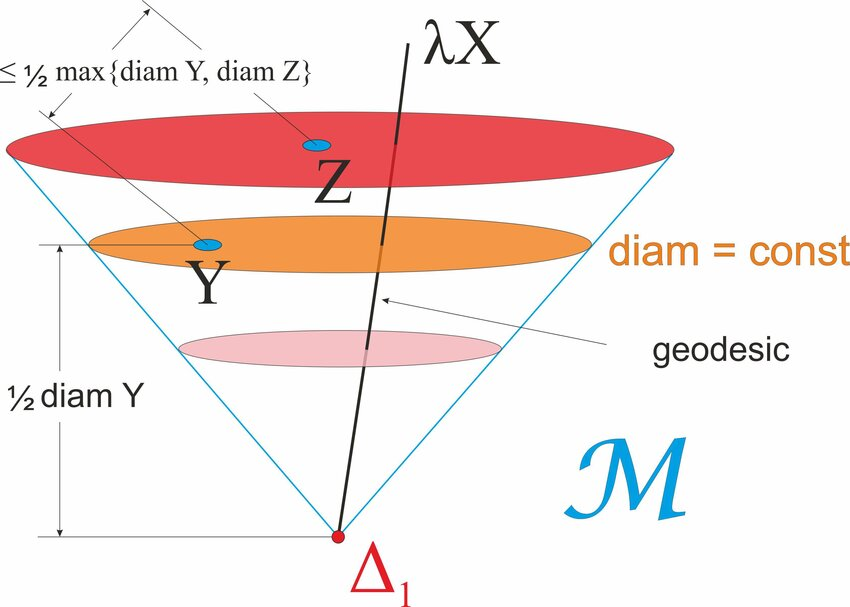
\includegraphics[width=0.7\linewidth]{Gromov-Hausdorff-space-general-properties.jpg}
    \label{fig:enter-label}
\end{figure}
}
\end{frame}

\begin{frame}[allowframebreaks]{Stabilizer group}
Multiplying spaces by \(\lambda > 0\) can produce interesting results. The distance $|X,\lambda X|$ can be infinite. For example, if $X$ is a geometric progression.

\textbf{Stabilizer group:} all $\lambda > 0$ such that $[X] = [\lambda X]$.

\textbf{Trivial:} $\St\left([X]\right) = \{1\}$.

\textbf{Center:} metric space $X$, such that $X = \lambda X$ \\for all $\lambda \in \St([X])$.
\end{frame}

\begin{frame}[allowframebreaks]{Gromov--Hausdorff distance between clouds}
Metric spaces are \underline{sets} by definition. 

Clouds are not sets, they are \underline{proper classes}. They contain sets of arbitrary cardinality.

Definition of Gromov--Hausdorff distance is modified.
\end{frame}

\begin{frame}[allowframebreaks]{Center image Theorem}
Clouds $[M], [\Delta_1]$, $[M]$ has a nontrivial stabilizer and $M$ --- center. $R$ --- correspondence between them, $\dis R = \epsilon < \infty$. Then  $\big|R(\Delta_1), M\big| \le 2\epsilon$.
\end{frame}

\begin{frame}[allowframebreaks]{Center image Theorem}
\tikzset{every picture/.style={line width=0.75pt}} %set default line width to 0.75pt        
\centering
\scalebox{0.7}{      

\begin{tikzpicture}[x=0.75pt,y=0.75pt,yscale=-1,xscale=1]
%uncomment if require: \path (0,921); %set diagram left start at 0, and has height of 921

%Straight Lines [id:da46864569152477] 
\draw    (166.8,142.95) -- (368.8,142.95) ;
\draw [shift={(370.8,142.95)}, rotate = 180] [color={rgb, 255:red, 0; green, 0; blue, 0 }  ][line width=0.75]    (10.93,-3.29) .. controls (6.95,-1.4) and (3.31,-0.3) .. (0,0) .. controls (3.31,0.3) and (6.95,1.4) .. (10.93,3.29)   ;
%Straight Lines [id:da9079407164606472] 
\draw    (166.8,306.95) -- (369.8,306.95) ;
\draw [shift={(371.8,306.95)}, rotate = 180] [color={rgb, 255:red, 0; green, 0; blue, 0 }  ][line width=0.75]    (10.93,-3.29) .. controls (6.95,-1.4) and (3.31,-0.3) .. (0,0) .. controls (3.31,0.3) and (6.95,1.4) .. (10.93,3.29)   ;
%Straight Lines [id:da3795104888549109] 
\draw    (154.8,184.95) -- (154.8,307.95) ;
\draw [shift={(154.8,307.95)}, rotate = 90] [color={rgb, 255:red, 0; green, 0; blue, 0 }  ][fill={rgb, 255:red, 0; green, 0; blue, 0 }  ][line width=0.75]      (0, 0) circle [x radius= 3.35, y radius= 3.35]   ;
\draw [shift={(154.8,184.95)}, rotate = 90] [color={rgb, 255:red, 0; green, 0; blue, 0 }  ][fill={rgb, 255:red, 0; green, 0; blue, 0 }  ][line width=0.75]      (0, 0) circle [x radius= 3.35, y radius= 3.35]   ;
%Straight Lines [id:da8627009276076836] 
\draw    (154.8,102.95) -- (154.8,143.95) ;
\draw [shift={(154.8,143.95)}, rotate = 90] [color={rgb, 255:red, 0; green, 0; blue, 0 }  ][fill={rgb, 255:red, 0; green, 0; blue, 0 }  ][line width=0.75]      (0, 0) circle [x radius= 3.35, y radius= 3.35]   ;
\draw [shift={(154.8,102.95)}, rotate = 90] [color={rgb, 255:red, 0; green, 0; blue, 0 }  ][fill={rgb, 255:red, 0; green, 0; blue, 0 }  ][line width=0.75]      (0, 0) circle [x radius= 3.35, y radius= 3.35]   ;
%Straight Lines [id:da2066957974184357] 
\draw    (154.8,143.95) -- (154.8,184.95) ;
%Straight Lines [id:da051691538152860095] 
\draw    (382.8,183.95) -- (383.8,306.95) ;
\draw [shift={(383.8,306.95)}, rotate = 89.53] [color={rgb, 255:red, 0; green, 0; blue, 0 }  ][fill={rgb, 255:red, 0; green, 0; blue, 0 }  ][line width=0.75]      (0, 0) circle [x radius= 3.35, y radius= 3.35]   ;
\draw [shift={(382.8,183.95)}, rotate = 89.53] [color={rgb, 255:red, 0; green, 0; blue, 0 }  ][fill={rgb, 255:red, 0; green, 0; blue, 0 }  ][line width=0.75]      (0, 0) circle [x radius= 3.35, y radius= 3.35]   ;
%Straight Lines [id:da8270918287513566] 
\draw    (166.8,101.95) -- (368.8,101.95) ;
\draw [shift={(370.8,101.95)}, rotate = 180] [color={rgb, 255:red, 0; green, 0; blue, 0 }  ][line width=0.75]    (10.93,-3.29) .. controls (6.95,-1.4) and (3.31,-0.3) .. (0,0) .. controls (3.31,0.3) and (6.95,1.4) .. (10.93,3.29)   ;
%Straight Lines [id:da7464347787216726] 
\draw    (166.8,183.95) -- (368.8,183.95) ;
\draw [shift={(370.8,183.95)}, rotate = 180] [color={rgb, 255:red, 0; green, 0; blue, 0 }  ][line width=0.75]    (10.93,-3.29) .. controls (6.95,-1.4) and (3.31,-0.3) .. (0,0) .. controls (3.31,0.3) and (6.95,1.4) .. (10.93,3.29)   ;
%Straight Lines [id:da8358695556916239] 
\draw    (382.8,101.95) -- (382.8,142.95) ;
\draw [shift={(382.8,142.95)}, rotate = 90] [color={rgb, 255:red, 0; green, 0; blue, 0 }  ][fill={rgb, 255:red, 0; green, 0; blue, 0 }  ][line width=0.75]      (0, 0) circle [x radius= 3.35, y radius= 3.35]   ;
\draw [shift={(382.8,101.95)}, rotate = 90] [color={rgb, 255:red, 0; green, 0; blue, 0 }  ][fill={rgb, 255:red, 0; green, 0; blue, 0 }  ][line width=0.75]      (0, 0) circle [x radius= 3.35, y radius= 3.35]   ;
%Straight Lines [id:da5038925133469215] 
\draw    (382.8,142.95) -- (382.8,183.95) ;
%Shape: Brace [id:dp7372340241482547] 
\draw   (428.8,304.95) .. controls (433.47,304.92) and (435.79,302.58) .. (435.76,297.91) -- (435.36,233.41) .. controls (435.32,226.74) and (437.63,223.39) .. (442.3,223.36) .. controls (437.63,223.39) and (435.28,220.08) .. (435.24,213.41)(435.26,216.41) -- (434.85,148.91) .. controls (434.82,144.24) and (432.47,141.92) .. (427.8,141.95) ;
%Straight Lines [id:da5006794443694909] 
\draw    (383.8,306.95) -- (383.8,384.95) ;
\draw [shift={(383.8,384.95)}, rotate = 90] [color={rgb, 255:red, 0; green, 0; blue, 0 }  ][fill={rgb, 255:red, 0; green, 0; blue, 0 }  ][line width=0.75]      (0, 0) circle [x radius= 3.35, y radius= 3.35]   ;
%Straight Lines [id:da650122086988841] 
\draw    (154.8,102.95) -- (154.8,17.95) ;
\draw [shift={(154.8,15.95)}, rotate = 90] [color={rgb, 255:red, 0; green, 0; blue, 0 }  ][line width=0.75]    (10.93,-3.29) .. controls (6.95,-1.4) and (3.31,-0.3) .. (0,0) .. controls (3.31,0.3) and (6.95,1.4) .. (10.93,3.29)   ;

% Text Node
\draw (108,293) node [anchor=north west][inner sep=0.75pt]   [align=left] {$\displaystyle \Delta _{1}$};
% Text Node
\draw (123,132) node [anchor=north west][inner sep=0.75pt]   [align=left] {$\displaystyle X$};
% Text Node
\draw (393,129.36) node [anchor=north west][inner sep=0.75pt]   [align=left] {$\displaystyle kY$};
% Text Node
\draw (400,295.29) node [anchor=north west][inner sep=0.75pt]   [align=left] {$\displaystyle Y$};
% Text Node
\draw (445,211.81) node [anchor=north west][inner sep=0.75pt]   [align=left] {$\displaystyle \rho $};
% Text Node
\draw (399,373.59) node [anchor=north west][inner sep=0.75pt]   [align=left] {$\displaystyle M$};
% Text Node
\draw (401,332.9) node [anchor=north west][inner sep=0.75pt]   [align=left] {$\displaystyle d$};
% Text Node
\draw (77,92) node [anchor=north west][inner sep=0.75pt]   [align=left] {$\displaystyle ( 1+\alpha ) X$};
% Text Node
\draw (78,174) node [anchor=north west][inner sep=0.75pt]   [align=left] {$\displaystyle ( 1-\beta ) X$};
% Text Node
\draw (392,172) node [anchor=north west][inner sep=0.75pt]   [align=left] {$\displaystyle kY_{\beta }$};
% Text Node
\draw (394,90) node [anchor=north west][inner sep=0.75pt]   [align=left] {$\displaystyle kY_{\alpha }$};

\end{tikzpicture}
}
\end{frame}

\begin{frame}[allowframebreaks]{Center image Theorem}
\tikzset{every picture/.style={line width=0.75pt}} %set default line width to 0.75pt        
\scalebox{0.7}{
\begin{tikzpicture}[x=0.75pt,y=0.75pt,yscale=-1,xscale=1]
%uncomment if require: \path (0,921); %set diagram left start at 0, and has height of 921

%Straight Lines [id:da44816903577612965] 
\draw    (156.8,574.55) -- (358.8,574.55) ;
\draw [shift={(360.8,574.55)}, rotate = 180] [color={rgb, 255:red, 0; green, 0; blue, 0 }  ][line width=0.75]    (10.93,-3.29) .. controls (6.95,-1.4) and (3.31,-0.3) .. (0,0) .. controls (3.31,0.3) and (6.95,1.4) .. (10.93,3.29)   ;
%Straight Lines [id:da8855594401963037] 
\draw    (142.8,533.55) -- (142.8,574.55) ;
\draw [shift={(142.8,574.55)}, rotate = 90] [color={rgb, 255:red, 0; green, 0; blue, 0 }  ][fill={rgb, 255:red, 0; green, 0; blue, 0 }  ][line width=0.75]      (0, 0) circle [x radius= 3.35, y radius= 3.35]   ;
\draw [shift={(142.8,533.55)}, rotate = 90] [color={rgb, 255:red, 0; green, 0; blue, 0 }  ][fill={rgb, 255:red, 0; green, 0; blue, 0 }  ][line width=0.75]      (0, 0) circle [x radius= 3.35, y radius= 3.35]   ;
%Straight Lines [id:da5328910089868972] 
\draw    (142.8,574.55) -- (142.8,615.55) ;
\draw [shift={(142.8,615.55)}, rotate = 90] [color={rgb, 255:red, 0; green, 0; blue, 0 }  ][fill={rgb, 255:red, 0; green, 0; blue, 0 }  ][line width=0.75]      (0, 0) circle [x radius= 3.35, y radius= 3.35]   ;
%Straight Lines [id:da4010896186693913] 
\draw    (156.8,533.55) -- (358.8,533.55) ;
\draw [shift={(360.8,533.55)}, rotate = 180] [color={rgb, 255:red, 0; green, 0; blue, 0 }  ][line width=0.75]    (10.93,-3.29) .. controls (6.95,-1.4) and (3.31,-0.3) .. (0,0) .. controls (3.31,0.3) and (6.95,1.4) .. (10.93,3.29)   ;
%Straight Lines [id:da21828437045013538] 
\draw    (156.8,615.55) -- (358.8,615.55) ;
\draw [shift={(360.8,615.55)}, rotate = 180] [color={rgb, 255:red, 0; green, 0; blue, 0 }  ][line width=0.75]    (10.93,-3.29) .. controls (6.95,-1.4) and (3.31,-0.3) .. (0,0) .. controls (3.31,0.3) and (6.95,1.4) .. (10.93,3.29)   ;
%Straight Lines [id:da736424125888303] 
\draw    (370.8,532.55) -- (370.8,573.55) ;
\draw [shift={(370.8,573.55)}, rotate = 90] [color={rgb, 255:red, 0; green, 0; blue, 0 }  ][fill={rgb, 255:red, 0; green, 0; blue, 0 }  ][line width=0.75]      (0, 0) circle [x radius= 3.35, y radius= 3.35]   ;
\draw [shift={(370.8,532.55)}, rotate = 90] [color={rgb, 255:red, 0; green, 0; blue, 0 }  ][fill={rgb, 255:red, 0; green, 0; blue, 0 }  ][line width=0.75]      (0, 0) circle [x radius= 3.35, y radius= 3.35]   ;
%Straight Lines [id:da526665799008399] 
\draw    (370.8,573.55) -- (370.8,614.55) ;
%Straight Lines [id:da5651829651425702] 
\draw    (142.8,533.55) -- (142.8,448.55) ;
\draw [shift={(142.8,446.55)}, rotate = 90] [color={rgb, 255:red, 0; green, 0; blue, 0 }  ][line width=0.75]    (10.93,-3.29) .. controls (6.95,-1.4) and (3.31,-0.3) .. (0,0) .. controls (3.31,0.3) and (6.95,1.4) .. (10.93,3.29)   ;
%Straight Lines [id:da4218697562628433] 
\draw    (370.8,614.55) -- (370.8,685.15) ;
\draw [shift={(370.8,685.15)}, rotate = 90] [color={rgb, 255:red, 0; green, 0; blue, 0 }  ][fill={rgb, 255:red, 0; green, 0; blue, 0 }  ][line width=0.75]      (0, 0) circle [x radius= 3.35, y radius= 3.35]   ;
\draw [shift={(370.8,614.55)}, rotate = 90] [color={rgb, 255:red, 0; green, 0; blue, 0 }  ][fill={rgb, 255:red, 0; green, 0; blue, 0 }  ][line width=0.75]      (0, 0) circle [x radius= 3.35, y radius= 3.35]   ;
%Straight Lines [id:da14640180624484178] 
\draw    (142.8,615.55) -- (142.8,697.55) ;
\draw [shift={(142.8,699.55)}, rotate = 270] [color={rgb, 255:red, 0; green, 0; blue, 0 }  ][line width=0.75]    (10.93,-3.29) .. controls (6.95,-1.4) and (3.31,-0.3) .. (0,0) .. controls (3.31,0.3) and (6.95,1.4) .. (10.93,3.29)   ;

% Text Node
\draw (385,560.96) node [anchor=north west][inner sep=0.75pt]   [align=left] {$\displaystyle Y$};
% Text Node
\draw (106,519.6) node [anchor=north west][inner sep=0.75pt]   [align=left] {$\displaystyle X_{\alpha }$};
% Text Node
\draw (107,604.6) node [anchor=north west][inner sep=0.75pt]   [align=left] {$\displaystyle X_{\beta }$};
% Text Node
\draw (384,603.6) node [anchor=north west][inner sep=0.75pt]   [align=left] {$\displaystyle Y_{\beta }$};
% Text Node
\draw (386,521.6) node [anchor=north west][inner sep=0.75pt]   [align=left] {$\displaystyle Y_{\alpha }$};
% Text Node
\draw (106,561.96) node [anchor=north west][inner sep=0.75pt]   [align=left] {$\displaystyle \Delta _{1}$};
% Text Node
\draw (385,674.59) node [anchor=north west][inner sep=0.75pt]   [align=left] {$\displaystyle M$};


\end{tikzpicture}


}
\end{frame}

\begin{frame}[allowframebreaks]{Distance theorem}
A cloud has a \underline{nontrivial} stabilizer, and there are two spaces which break the ultrametric inequality. Then it's distance to $[\Delta_1]$ is \underline{infinite}.

$M$ is the center of $[M]$, $Y_1$ and $Y_2$ are such metric spaces that 
\begin{gather*}
    |Y_1, M| \le \rho,\\
    |Y_1,M| \le \rho,\\
    |Y_1,Y_2| > \rho.
\end{gather*}
\end{frame}

\begin{frame}[allowframebreaks]{Distance Theorem}
\[X_1 = R^{-1}(Y_1), X_2 = R^{-1}(Y_2)\]
\scalebox{0.7}{

\begin{tikzpicture}[x=0.75pt,y=0.75pt,yscale=-1,xscale=1]
%uncomment if require: \path (0,1249); %set diagram left start at 0, and has height of 1249

%Straight Lines [id:da5227304211725639] 
\draw    (62.8,832.15) -- (229.8,932.15) ;
\draw [shift={(229.8,932.15)}, rotate = 30.91] [color={rgb, 255:red, 0; green, 0; blue, 0 }  ][fill={rgb, 255:red, 0; green, 0; blue, 0 }  ][line width=0.75]      (0, 0) circle [x radius= 3.35, y radius= 3.35]   ;
\draw [shift={(62.8,832.15)}, rotate = 30.91] [color={rgb, 255:red, 0; green, 0; blue, 0 }  ][fill={rgb, 255:red, 0; green, 0; blue, 0 }  ][line width=0.75]      (0, 0) circle [x radius= 3.35, y radius= 3.35]   ;
%Straight Lines [id:da3536854321424038] 
\draw    (62.8,832.15) -- (229.8,1001.15) ;
%Straight Lines [id:da22783116834497008] 
\draw    (396.8,832.15) -- (229.8,932.15) ;
\draw [shift={(396.8,832.15)}, rotate = 149.09] [color={rgb, 255:red, 0; green, 0; blue, 0 }  ][fill={rgb, 255:red, 0; green, 0; blue, 0 }  ][line width=0.75]      (0, 0) circle [x radius= 3.35, y radius= 3.35]   ;
%Straight Lines [id:da17835458744987787] 
\draw    (396.8,832.15) -- (229.8,1001.15) ;
\draw [shift={(229.8,1001.15)}, rotate = 134.66] [color={rgb, 255:red, 0; green, 0; blue, 0 }  ][fill={rgb, 255:red, 0; green, 0; blue, 0 }  ][line width=0.75]      (0, 0) circle [x radius= 3.35, y radius= 3.35]   ;
\draw [shift={(396.8,832.15)}, rotate = 134.66] [color={rgb, 255:red, 0; green, 0; blue, 0 }  ][fill={rgb, 255:red, 0; green, 0; blue, 0 }  ][line width=0.75]      (0, 0) circle [x radius= 3.35, y radius= 3.35]   ;
%Straight Lines [id:da8543112602327929] 
\draw    (229.8,998.15) -- (229.8,935.15) ;
\draw [shift={(229.8,932.15)}, rotate = 90] [fill={rgb, 255:red, 0; green, 0; blue, 0 }  ][line width=0.08]  [draw opacity=0] (8.93,-4.29) -- (0,0) -- (8.93,4.29) -- cycle    ;
\draw [shift={(229.8,1001.15)}, rotate = 270] [fill={rgb, 255:red, 0; green, 0; blue, 0 }  ][line width=0.08]  [draw opacity=0] (8.93,-4.29) -- (0,0) -- (8.93,4.29) -- cycle    ;

% Text Node
\draw (48,799.55) node [anchor=north west][inner sep=0.75pt]   [align=left] {$\displaystyle X_{1}$};
% Text Node
\draw (385,796.55) node [anchor=north west][inner sep=0.75pt]   [align=left] {$\displaystyle X_{2}$};
% Text Node
\draw (202,886.55) node [anchor=north west][inner sep=0.75pt]   [align=left] {$\displaystyle R^{-1}( M)$};
% Text Node
\draw (218,1011.55) node [anchor=north west][inner sep=0.75pt]   [align=left] {$\displaystyle \Delta _{1}$};
% Text Node
\draw (235,945.55) node [anchor=north west][inner sep=0.75pt]   [align=left] {$\displaystyle 2\epsilon $};


\end{tikzpicture}


}
\end{frame}


% ***************
% ***** END *****
% ***************

\end{document}
